\section{密度的存在性}
\label{sec:density-existence}

上一节得到一个必要条件：$\nu$若有相对于$\mu$的密度，就必有$\nu\ll\mu$。本节证明，在两个测度都$\sigma$有限时这个条件也是充分的，并且密度在$\mu$-几乎处处意义下唯一。然后把这个结论用到第~\ref{sec:measure-decomposition}节的Lebesgue分解上，看清一个测度中哪一部分能用密度表示、哪一部分不能；最后把密度推广到有限有符号测度。

\subsection{Radon–Nikodym定理}
\label{sec:density-radon-nikodym}

绝对连续只是一个关于零测集的条件：$\mu$看不见的集合，$\nu$也看不见。它并没有直接给出任何函数。要从$\nu$在所有集合上的质量中“反求”一个逐点权重，必须同时满足不可数多个集合上的等式，这正是定理的难处。

\begin{theorem}[Radon–Nikodym定理]
\label{thm:density-radon-nikodym}
设$\mu,\nu$是可测空间$(X,\mathcal A)$上的$\sigma$有限非负测度，且$\nu\ll\mu$。则存在可测函数$h:X\to[0,+\infty)$，使
\[
 \nu(A)=\int_Ah\,\mathrm d\mu,\qquad A\in\mathcal A .
\]
若可测函数$g:X\to[0,+\infty]$也满足这一等式，则$g=h$ $\mu$-几乎处处。
\end{theorem}

把\term{Radon–Nikodym定理}（Radon-Nikodym theorem）与定理~\ref{thm:density-weighted-measure}对照：那里从$h$出发得到测度，这里从测度出发得到$h$。结合两者，在$\sigma$有限范围内，“$\nu$相对于$\mu$有密度”与“$\nu\ll\mu$”是同一件事。证明先处理两个测度都有限的情形，再用$\sigma$有限性把空间切成可数个有限块。

\paragraph{有限情形：候选权重取最大}
思路是在所有“不超过$\nu$”的权重中找一个最大的。直观上，若某个权重在每个集合上产生的质量都不超过$\nu$，而它已经大到不能再加高，那么它产生的质量就应该恰好等于$\nu$。

\begin{lemma}[有限测度的密度存在]
\label{lem:density-rn-finite}
设$\mu,\nu$是$(X,\mathcal A)$上的有限非负测度，且$\nu\ll\mu$。则存在可测函数$h:X\to[0,+\infty)$，使$\nu(A)=\int_Ah\,\mathrm d\mu$对一切$A\in\mathcal A$成立。
\end{lemma}

\begin{proof}
\emph{第一步：候选集合对取最大值封闭。}令
\[
 \mathcal G=\Bigl\{g:X\to[0,+\infty]\text{ 可测}:\ \int_Ag\,\mathrm d\mu\le\nu(A)\ \text{对一切}A\in\mathcal A\Bigr\}.
\]
$0\in\mathcal G$，所以$\mathcal G$非空。设$g_1,g_2\in\mathcal G$，$g=\max(g_1,g_2)$。对任意$A$，令$A_1=A\cap\{g_1\ge g_2\}$，$A_2=A\cap\{g_1<g_2\}$，二者可测、不交且并为$A$。在$A_1$上$g=g_1$，在$A_2$上$g=g_2$，于是
\[
 \int_Ag\,\mathrm d\mu=\int_{A_1}g_1\,\mathrm d\mu+\int_{A_2}g_2\,\mathrm d\mu\le\nu(A_1)+\nu(A_2)=\nu(A),
\]
故$g\in\mathcal G$。归纳可知有限个候选的最大值仍是候选。

\emph{第二步：用单调序列达到上确界。}令$s=\sup_{g\in\mathcal G}\int_Xg\,\mathrm d\mu$。每个候选满足$\int_Xg\,\mathrm d\mu\le\nu(X)$，所以$s\le\nu(X)<\infty$。取$g_n\in\mathcal G$使$\int_Xg_n\,\mathrm d\mu\to s$，再令$h_n=\max(g_1,\dots,g_n)$。由第一步$h_n\in\mathcal G$；$h_n$关于$n$单调递增，且$h_n\ge g_n$，所以$\int_Xg_n\,\mathrm d\mu\le\int_Xh_n\,\mathrm d\mu\le s$。令$h=\lim_nh_n$，它是可测函数。对每个$A$，$h_n\mathbf 1_A$递增到$h\mathbf 1_A$，单调收敛定理给出
\[
 \int_Ah\,\mathrm d\mu=\lim_{n\to\infty}\int_Ah_n\,\mathrm d\mu\le\nu(A),
\]
所以$h\in\mathcal G$；取$A=X$并由夹逼得$\int_Xh\,\mathrm d\mu=s$。上确界由一个候选达到，只用到了可数个候选，这正是单调收敛定理能够处理的情形。由于$\int_Xh\,\mathrm d\mu<\infty$，$h$只在一个$\mu$零测集上取$+\infty$；把这些值改为$0$不改变任何集合上的积分（第~\ref{sec:density-ae-version}小节），所以可设$h$处处有限。

\emph{第三步：剩余质量为零。}令$r(A)=\nu(A)-\int_Ah\,\mathrm d\mu$。因$h\in\mathcal G$，$r(A)\ge0$；$\nu$与$\nu_h$（定理~\ref{thm:density-weighted-measure}）都是有限测度，两个收敛级数逐项相减，可知$r$可数可加，是有限非负测度；又$r(A)\le\nu(A)$，所以$r\ll\mu$。反设$r(X)>0$。由$r\ll\mu$知$\mu(X)>0$，取
\[
 \varepsilon=\frac{r(X)}{2\mu(X)}>0,
\]
则$(r-\varepsilon\mu)(X)=r(X)/2>0$。$r-\varepsilon\mu$是两个有限测度之差，是有限有符号测度（定义~\ref{def:measure-signed}）。由Hahn分解（定理~\ref{thm:measure-hahn}），存在可测集$P$，使$P$是$r-\varepsilon\mu$的正集，$N=X\setminus P$是负集。

先说明$P$不是$\mu$零测集。$(r-\varepsilon\mu)(N)\le0$，所以$(r-\varepsilon\mu)(P)\ge(r-\varepsilon\mu)(X)>0$，从而$r(P)>\varepsilon\mu(P)\ge0$；再由$r\ll\mu$得$\mu(P)>0$。再说明在$h$上加高$\varepsilon\mathbf 1_P$仍是候选。对任意$A$，$A\cap P$是正集$P$的可测子集，于是$\varepsilon\mu(A\cap P)\le r(A\cap P)\le r(A)$，进而
\[
 \int_A(h+\varepsilon\mathbf 1_P)\,\mathrm d\mu=\int_Ah\,\mathrm d\mu+\varepsilon\mu(A\cap P)\le\int_Ah\,\mathrm d\mu+r(A)=\nu(A).
\]
所以$h+\varepsilon\mathbf 1_P\in\mathcal G$，但它的总积分为$s+\varepsilon\mu(P)>s$，与$s$是上确界矛盾。因此$r(X)=0$；由$0\le r(A)\le r(X)$，$r$在每个集合上为零，即$\nu(A)=\int_Ah\,\mathrm d\mu$。
\end{proof}

图~\ref{fig:density-rn-candidate}用一个事后已知密度$f$的例子示意第三步。蓝色候选$h$在左半段低于$f$，两者之间的黄色区域是尚未被表示的剩余质量$r$。Hahn分解找出的正集$P$，正是剩余质量“至少有$\varepsilon$倍长度”的地方；在那里把$h$加高$\varepsilon$，绿色条带仍在$f$之下，所以加高后仍是候选。只要剩余质量不为零，就总能这样再加高一点，最大的候选因而不留下任何剩余。

\begin{figure}[!htbp]
  \centering
  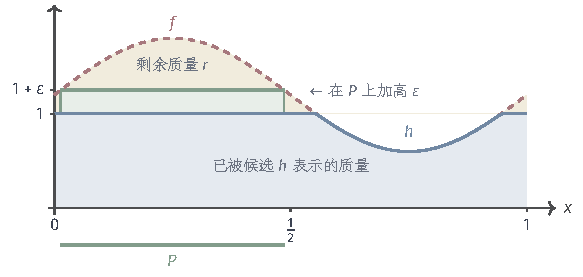
\includegraphics[width=98.771mm]{figures/02-abstract-mathematics/01-metric-and-measure/tikz/c4-rn-candidate/figure.pdf}
  \caption{有限情形证明第三步的示意。参考测度为$[0,1]$上的长度，目标测度的密度$f(x)=1.2+0.6\sin(2\pi x)$（红色虚线）在证明中事先未知，这里画出只为便于观察。候选$h=\min(f,1)$（蓝色实线）之下的质量已被表示，$h$与$f$之间的黄色区域是剩余质量$r$。取$\varepsilon=0.25$，正集$P=\{f-h\ge\varepsilon\}$约为$[0.013,0.487]$；在$P$上加高$\varepsilon$的绿色条带仍在$f$之下，所以$h+\varepsilon\mathbf 1_P$仍是候选而总积分更大。}
  \label{fig:density-rn-candidate}
\end{figure}

\paragraph{$\sigma$有限情形与唯一性}
有限情形中，$\nu(X)<\infty$保证了上确界$s$有限，$\mu(X)<\infty$保证了$r-\varepsilon\mu$是有限有符号测度，从而可以用Hahn分解。对$\sigma$有限测度，先把空间切成两种测度都有限的小块。

\begin{proof}[定理~\ref{thm:density-radon-nikodym}的证明]
\emph{有限分块。}由$\sigma$有限性，存在两两不交的可测集$A_1,A_2,\dots$覆盖$X$且$\mu(A_i)<\infty$，以及两两不交的可测集$B_1,B_2,\dots$覆盖$X$且$\nu(B_j)<\infty$。集合族$\{A_i\cap B_j\}_{i,j}$可数、两两不交、覆盖$X$，并且每块上$\mu$与$\nu$都有限；把它们排成一列$X_1,X_2,\dots$。

\emph{存在性。}对每个$k$，令$\mu_k(A)=\mu(A\cap X_k)$，$\nu_k(A)=\nu(A\cap X_k)$。它们是有限测度，且$\mu_k(A)=0$时$\nu(A\cap X_k)=0$，即$\nu_k\ll\mu_k$。由引理~\ref{lem:density-rn-finite}，存在有限值可测函数$h_k$使$\nu_k(A)=\int_Ah_k\,\mathrm d\mu_k$。对非负可测$f$有$\int_Xf\,\mathrm d\mu_k=\int_Xf\mathbf 1_{X_k}\,\mathrm d\mu$：对示性函数$f=\mathbf 1_B$，两边都是$\mu(B\cap X_k)$；由线性性推广到非负简单函数，再由简单函数逼近（引理~\ref{lem:integral-simple-approx}）和单调收敛推广到一般非负可测函数。令
\[
 h=\sum_{k=1}^\infty h_k\mathbf 1_{X_k},
\]
因各$X_k$不交，每点处至多一项非零，$h$有限、可测。对任意$A$，由$\nu$的可数可加性和非负级数的逐项积分（单调收敛定理），
\[
 \nu(A)=\sum_{k=1}^\infty\nu(A\cap X_k)=\sum_{k=1}^\infty\int_Ah_k\mathbf 1_{X_k}\,\mathrm d\mu=\int_A\sum_{k=1}^\infty h_k\mathbf 1_{X_k}\,\mathrm d\mu=\int_Ah\,\mathrm d\mu .
\]

\emph{唯一性。}设$g:X\to[0,+\infty]$也满足$\nu(A)=\int_Ag\,\mathrm d\mu$。固定$k$。由于$\int_{X_k}h\,\mathrm d\mu=\int_{X_k}g\,\mathrm d\mu=\nu(X_k)<\infty$，$h\mathbf 1_{X_k}$与$g\mathbf 1_{X_k}$都可积。令$D=X_k\cap\{h>g\}$，则$\int_Dh\,\mathrm d\mu=\nu(D)=\int_Dg\,\mathrm d\mu$，两边有限，由可积函数积分的线性性，
\[
 \int_X(h-g)\mathbf 1_D\,\mathrm d\mu=0 .
\]
在$D$上$g<h<\infty$，所以被积函数$(h-g)\mathbf 1_D$有定义且非负；积分为零的非负函数几乎处处为零（第~\ref{sec:integral-properties}节）；而它在$D$上严格为正，所以$\mu(D)=0$。同理$\mu(X_k\cap\{g>h\})=0$。对$k$取可数并，$\{g\ne h\}$是$\mu$零测集。
\end{proof}

整个证明只用到第~\ref{chap:measures}章的测度运算与Hahn分解，以及第~\ref{chap:integration}章的积分基本性质和单调收敛定理，不需要函数空间的理论。从第二步还能读出密度的一个刻画：$\mathrm d\nu/\mathrm d\mu$是所有“在每个集合上都不超过$\nu$”的权重中积分最大的那个。

\subsection{密度表示与测度分解}
\label{sec:density-decomposition}

第~\ref{sec:measure-decomposition}节已经把一个$\sigma$有限测度$\nu$相对于参考测度$\mu$唯一地拆成$\nu=\nu_{\mathrm{ac}}+\nu_{\mathrm s}$，其中$\nu_{\mathrm{ac}}\ll\mu$、$\nu_{\mathrm s}\perp\mu$（定理~\ref{thm:measure-lebesgue-decomposition}）。那里只分开了两种质量，没有给绝对连续部分任何函数表示；Radon–Nikodym定理正好补上这一步。

\begin{theorem}[Lebesgue分解的密度形式（推论）]
\label{thm:density-lebesgue-form}
设$\mu,\nu$是$(X,\mathcal A)$上的$\sigma$有限非负测度。则存在可测函数$h:X\to[0,+\infty)$和非负测度$\nu_{\mathrm s}\perp\mu$，使
\[
 \nu(A)=\int_Ah\,\mathrm d\mu+\nu_{\mathrm s}(A),\qquad A\in\mathcal A,
\]
其中$\nu_{\mathrm s}$唯一，$h$在$\mu$-几乎处处意义下唯一。特别地，$\nu$相对于$\mu$有密度，当且仅当$\nu_{\mathrm s}=0$。
\end{theorem}

\begin{proof}
由定理~\ref{thm:measure-lebesgue-decomposition}得到$\nu=\nu_{\mathrm{ac}}+\nu_{\mathrm s}$。$\nu_{\mathrm{ac}}(A)\le\nu(A)$，所以覆盖$X$且$\nu$有限的可数块也使$\nu_{\mathrm{ac}}$有限，$\nu_{\mathrm{ac}}$是$\sigma$有限的。对$\nu_{\mathrm{ac}}\ll\mu$应用定理~\ref{thm:density-radon-nikodym}，得$h=\mathrm d\nu_{\mathrm{ac}}/\mathrm d\mu$。唯一性：若另有$(h',\nu_{\mathrm s}')$满足同样的表示，则$A\mapsto\int_Ah'\,\mathrm d\mu$绝对连续（定理~\ref{thm:density-weighted-measure}），由Lebesgue分解的唯一性，它等于$\nu_{\mathrm{ac}}$且$\nu_{\mathrm s}'=\nu_{\mathrm s}$；再由Radon–Nikodym定理中的唯一性得$h'=h$ $\mu$-几乎处处。最后，若$\nu$有密度，则$\nu\ll\mu$，$\nu=\nu+0$就是它的Lebesgue分解，所以$\nu_{\mathrm s}=0$；反之$\nu_{\mathrm s}=0$时$h$就是$\nu$的密度。
\end{proof}

两个定理的分工由此清楚：Lebesgue分解只用测度把参考测度能看见的质量与看不见的质量分开；Radon–Nikodym定理为前一部分找到逐点权重。奇异部分无论如何也写不成相对于$\mu$的密度，因为它集中在一个$\mu$零测集上，而任何密度在零测集上的积分都是$0$。

\paragraph{实轴上的三种质量}
以Lebesgue测度$\lambda$为参考时，第~\ref{sec:measure-decomposition}节把奇异部分进一步拆成点质量与没有点质量的奇异连续质量。考虑$[0,1]$上的概率测度
\[
 \nu=\tfrac12\lambda|_{[0,1]}+\tfrac14\delta_{1/2}+\tfrac14\mu_C,
\]
其中$\mu_C$是第~\ref{sec:measure-decomposition}节的Cantor测度，集中在Lebesgue零测的Cantor集$C$上。$\tfrac14\delta_{1/2}+\tfrac14\mu_C$集中在零测集$C\cup\{1/2\}$上，与$\lambda$相互奇异；$\tfrac12\lambda|_{[0,1]}$相对于$\lambda$绝对连续。由分解的唯一性，
\[
 \nu(A)=\int_A\tfrac12\mathbf 1_{[0,1]}\,\mathrm d\lambda+\tfrac14\delta_{1/2}(A)+\tfrac14\mu_C(A).
\]
图~\ref{fig:density-lebesgue-form}画出这三部分：只有高为$1/2$的蓝色区域是密度能表示的，红色箭头和绿色Cantor集上的质量都在密度之外。

\begin{figure}[!htbp]
  \centering
  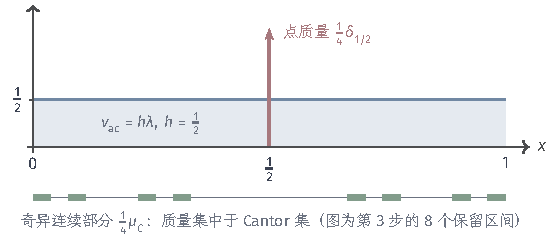
\includegraphics[width=94.365mm]{figures/02-abstract-mathematics/01-metric-and-measure/tikz/c4-lebesgue-density/figure.pdf}
  \caption{相对于长度测度的密度只表示绝对连续部分。$\nu=\tfrac12\lambda|_{[0,1]}+\tfrac14\delta_{1/2}+\tfrac14\mu_C$：蓝色区域是密度$h=1/2$表示的质量$1/2$；红色箭头是位于$1/2$的点质量$1/4$；下方绿色线段是Cantor集构造第$3$步保留的$8$个区间，Cantor测度的质量$1/4$集中在它们的极限——零长度的Cantor集上。后两部分都集中在长度零测集上，任何密度都无法表示。}
  \label{fig:density-lebesgue-form}
\end{figure}

由定理~\ref{thm:density-lebesgue-form}，$\nu$整体具有Lebesgue密度，当且仅当点质量部分与奇异连续部分都为零。累计函数$F(x)=\nu((-\infty,x])$的跳跃恰好读出点质量（第~\ref{sec:measure-construction}节），所以“$F$连续”只能排除点质量。Cantor测度的累计函数就是处处连续的Cantor函数，它却没有密度。判断密度是否存在，应当检查绝对连续性，而不是累计函数的连续性；第~\ref{sec:density-increment}小节还会从函数一侧回到这一点。

\paragraph{有限性条件不能随意去掉}
在$[0,1]$的Borel可测空间上取计数测度$c$与Lebesgue测度$\lambda$。$c(A)=0$只在$A=\varnothing$时成立，所以$\lambda\ll c$。若存在可测$h\ge0$使$\lambda(A)=\int_Ah\,\mathrm dc$，取$A=\{x\}$，$h\mathbf 1_{\{x\}}=h(x)\mathbf 1_{\{x\}}$是简单函数，于是
\[
 0=\lambda(\{x\})=h(x)\,c(\{x\})=h(x),\qquad x\in[0,1].
\]
$h$处处为零，却要给出$\lambda([0,1])=1$，矛盾。所以$\lambda$没有相对于$c$的密度。定理失效的原因在于参考测度：$c$的有限测度集只能是有限集，可数个有限集的并仍是可数集，盖不住$[0,1]$，所以$c$不是$\sigma$有限的。$\lambda$本身有限，第~\ref{sec:measure-decomposition}节的Lebesgue分解对它照常成立，给出$\lambda_{\mathrm{ac}}=\lambda$、$\lambda_{\mathrm s}=0$；失败的只是“为绝对连续部分找函数”这一步。

\begin{figure}[!htbp]
  \centering
  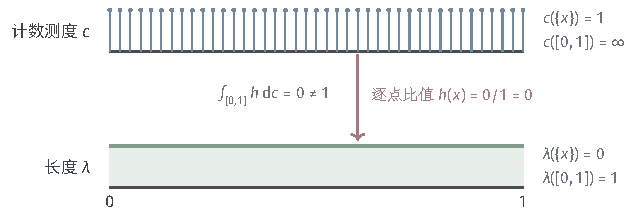
\includegraphics[width=107.636mm]{figures/02-abstract-mathematics/01-metric-and-measure/tikz/c4-counting-counterexample/figure.pdf}
  \caption{参考测度不$\sigma$有限时密度可能不存在。上方的计数测度$c$给$[0,1]$中每一点质量$1$（图中只画出若干点），下方的长度$\lambda$给单点质量$0$、给整个区间质量$1$。若$\lambda$有相对于$c$的密度，逐点比较单点质量迫使密度处处为$0$，其积分为$0$，不能恢复$\lambda([0,1])=1$。}
  \label{fig:density-counting-counterexample}
\end{figure}

这个反例说明定理不能无条件推广，但不说明$\sigma$有限是密度存在的必要条件。仍以不$\sigma$有限的$c$为参考，$\delta_0$有密度$\mathbf 1_{\{0\}}$：$\int_A\mathbf 1_{\{0\}}\,\mathrm dc=c(A\cap\{0\})=\delta_0(A)$。$\sigma$有限是本章采用的一组充分条件。图~\ref{fig:density-counting-counterexample}直观地显示了反例中失败的原因：参考测度的质量分得太“碎”，每一点都有正质量，任何逐点权重都只能逐点地复制目标测度在单点上的质量，而$\lambda$的质量恰恰不在任何单点上。

\subsection{有符号测度的密度}
\label{sec:density-signed}

第~\ref{sec:measure-signed}节的有限有符号测度允许集合质量为负。它同样可以用一个函数表示，只不过这个函数可以取负值，正负部分别对应Jordan分解的两项。

\begin{theorem}[有符号测度的密度]
\label{thm:density-signed}
设$\mu$是$(X,\mathcal A)$上的$\sigma$有限非负测度，$\eta$是有限有符号测度。则$|\eta|\ll\mu$当且仅当存在$\mu$可积的实值函数$h$，使
\[
 \eta(A)=\int_Ah\,\mathrm d\mu,\qquad A\in\mathcal A .
\]
此时$h$在$\mu$-几乎处处意义下唯一，并且对一切$A\in\mathcal A$，
\[
 \eta^+(A)=\int_Ah^+\,\mathrm d\mu,\qquad \eta^-(A)=\int_Ah^-\,\mathrm d\mu,\qquad |\eta|(A)=\int_A|h|\,\mathrm d\mu,
\]
其中$h^+=\max(h,0)$，$h^-=\max(-h,0)$。
\end{theorem}

\begin{proof}
设$|\eta|\ll\mu$。由Jordan分解（定理~\ref{thm:measure-jordan}），$\eta=\eta^+-\eta^-$，且$\eta^\pm\le\eta^++\eta^-=|\eta|$（定义~\ref{def:measure-total-variation}），所以$\eta^\pm\ll\mu$。$\eta^\pm$是有限测度，当然$\sigma$有限；由定理~\ref{thm:density-radon-nikodym}，存在有限值密度$h_1=\mathrm d\eta^+/\mathrm d\mu$与$h_2=\mathrm d\eta^-/\mathrm d\mu$，且$\int_Xh_1\,\mathrm d\mu=\eta^+(X)<\infty$，$h_2$同理，二者都可积。令$h=h_1-h_2$，由可积函数积分的线性性，$\eta(A)=\int_Ah_1\,\mathrm d\mu-\int_Ah_2\,\mathrm d\mu=\int_Ah\,\mathrm d\mu$。

反过来，设$\eta(A)=\int_Ah\,\mathrm d\mu$且$h$可积。令$P=\{h\ge0\}$，$N=\{h<0\}$。对$P$的任意可测子集$A$，$\eta(A)=\int_Ah\,\mathrm d\mu\ge0$；对$N$的任意可测子集，$\eta(A)\le0$。所以$(P,N)$是$\eta$的一组Hahn分解，由Jordan分解得
\[
 \begin{aligned}
  \eta^+(A)&=\eta(A\cap P)=\int_Ah\mathbf 1_{\{h\ge0\}}\,\mathrm d\mu=\int_Ah^+\,\mathrm d\mu,\\
  \eta^-(A)&=-\eta(A\cap N)=\int_Ah^-\,\mathrm d\mu,
 \end{aligned}
\]
相加得$|\eta|(A)=\int_A(h^++h^-)\,\mathrm d\mu=\int_A|h|\,\mathrm d\mu$。由定理~\ref{thm:density-weighted-measure}，$|\eta|\ll\mu$。这一段对前一段构造的$h$同样适用，所以三个公式在必要性方向也成立。

唯一性：若可积的$h,g$都表示$\eta$，则对$D=\{h>g\}$有$\int_X(h-g)\mathbf 1_D\,\mathrm d\mu=\eta(D)-\eta(D)=0$，非负被积函数几乎处处为零，所以$\mu(D)=0$；同理$\mu(\{g>h\})=0$。
\end{proof}

定理把集合层面的正负分解翻译成函数层面的正负部分：Hahn分解的正区域可以取为$\{h\ge0\}$，Jordan的两项就是$h$的正部与负部分别产生的测度，这与第~\ref{chap:integration}章用正负部定义实值函数积分的做法一致。总变差对应$|h|$的积分，所以“$\eta$有有限总变差且对$\mu$绝对连续”恰好对应“密度绝对可积”。

\paragraph{抵消与总变差}
在$[0,1]$上取$\mu=\lambda|_{[0,1]}$与$h(x)=1-2x$，令$\eta(A)=\int_Ah\,\mathrm d\lambda$。整体上$\eta([0,1])=\int_0^1(1-2x)\,\mathrm dx=0$，正负质量完全抵消。由定理，正区域为$[0,1/2]$，
\[
 \eta^+([0,1])=\int_0^{1/2}(1-2x)\,\mathrm dx=\tfrac14,\qquad \eta^-([0,1])=\int_{1/2}^1(2x-1)\,\mathrm dx=\tfrac14,
\]
所以$|\eta|([0,1])=\int_0^1|1-2x|\,\mathrm dx=\tfrac12$。$\eta(X)=0$并不说明$\eta$处处为零，总变差记录了被抵消掉的变化总量。第~\ref{sec:density-increment}小节将用这个定理表示由函数增量产生的有符号测度。
